\documentclass[12pt,fleqn]{article}\usepackage{../common}
\begin{document}
Ders 7

Ozel form

\[ y' + ky = kq_e(t) \]

Su cozulunce

\[ y'+ky = q(t) \]

su elde edilir

\[ y = e^{-kt} \int q(t) e^{kt} dt + ce^{-kt}\]

Bu denklemdeki sag ilk $kt$ ve soldaki $-kt$ ust degerlerinin ters isaretli
oldugunu hatirlamanin iyi bir yolu $q(t) = 1$ olunca ic ve dis $e$
degerlerinin birbirini iptal etmesi ve bu sayede sonucun sabit bir sayi
olmasi.

$c$'yi iceren terim arti isaretinden sonra da (ustteki gibi)
koyulabilir. Ya da onun yerine entegrale sifir alt siniri ve $t$ fuzuli
(dummy) degiskeni verilerek tanimsiz entegral tanimli entegral haline de
getirilebilir. 

Bu denklemde, sadece ve sadece $k>0$ oldugu zaman, $t$ sonsuzluga giderken
$e^{-kt}$ sifira gider (ve $c$'nin ne oldugu farketmez), geri kalan

\[ y = e^{-kt} \int q(t) e^{kt} dt  \]

denklemi ise istikrarli konum (steady-state) cozumu olacaktir. 

Denklemdeki $c$ $y(0)$ degerini kullanir. 

Birkac cozumu grafiklersek soyle bir sonuc gorebiliriz. Sari renkli olan
istikrarli olan cozumdur, diger tum cozumler ona yaklasir. Peki sari renkli
olan grafigin ozel tarafi nedir? Aslinda yoktur, tum cozumler sariya degil,
birbirlerine yaklasirlar. Daha detaylandirmak gerekirse, aslinda bir degil,
birden fazla istikrarli cozum vardir. 

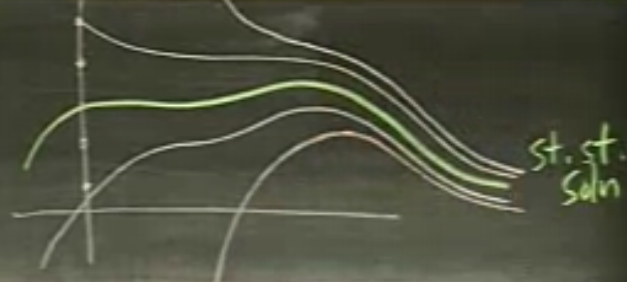
\includegraphics[height=4cm]{7_1.png}

O zaman hangi istikrarli cozumden bahsetmek gerekir?  $ce^{-kt}$'in sifira
gittigi en basit olani tabii ki, fakat $ce^{-kt}$'dan once gelen terim bir
sekilde $ce^{-kt}$ ile beraber daha basit bir formule de sebebiyet
verebilir. Yani duruma gore degisir. Genel olarak bizim en basit
erisebilecegimiz istikrarli cozum secilir. 

$q(t)$'yi bu problemde ``girdi'' olarak niteleyecegiz, cunku hep daha once
bahsettigimiz sicaklik problemini, ve o problemdeki $T_e$'yi dusunuyoruz,
$T_e$ havuza pompalanan bir sicaklik girdisi. 

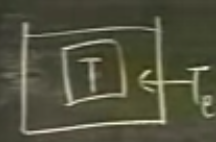
\includegraphics[height=2cm]{7_2.png}

Sistemin ``cevabi (response)'' ise diferansiyel denklemin cozumu $y(t)$. 

$q(t)$ yerine $q_e(t)$ kullanalim. 

Bu arada, bu denklemde girdilerin ust uste eklenebilmesi ozelligi vardir.

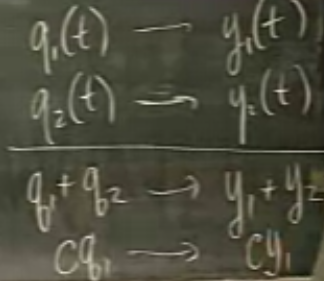
\includegraphics[height=4cm]{7_3.png}

$q_1+q_2$ birbirine eklenince sonuc $y_1+y_2$ olur. 

Soru: Eger girdi trigonometrik bir fonksiyon ise ne olur? Bu en onemli
durumdur (Fourier serilerinin mevcudiyeti sebebiyle, bu konuya ileride
girecegiz). 

\[ y' + ky = kq_e(t) \]

icin girdi olarak $cos(\omega t)$ verilmis. $\omega$ acisal frekans olarak
modelleniyor, yani $2\pi$ icinde kac tane tam salinimin (oscillation)
oldugu. $cos$ egrisini hatirlarsak, bir salinim 0 ile $2\pi$ arasindadir,
fonksiyon basladigi yere doner, salinim biter. $\omega$ ile salinim s�kligi
arttirilabilir, $\omega = 2$ ile 0 ile $2\pi$ arasinda iki kere tam salinim
olur. Yani frekans kelimesi burada biraz karisiklik yaratabilir, cunku
$2\pi$ icinde olanlara bakiyoruz, 1 birimlik zaman icinde neler olduguna
bakmiyoruz (ki bu frekansin cogunlukla kullanilan tanimidir). 

Problem

$q_e = \cos \omega t$ girdisini kullanarak cevabi hesapla (yani ODE'yi
coz). 

Cozum icin kompleks sayilari kullanacagiz. ODE'yi alip kompleks sayilari
kullanan bir hale cevirecegiz. Onu cozecegiz, sonra elimizdeki cevapla reel
sayilarin dunyasina donecegiz. Niye bu gecis? Cunku ustel fonksiyonlari
entegre etmek kolaydir. 

\[ e^{i\omega t} = \cos \omega t + i \sin \omega t \]

ODE'yi tekrar yazalim, girdiyi kompleks olarak yazalim

\[ y' + ky = k e^{i\omega t} \]

Fakat bunu yapinca tum $y$'lerin kompleks hale geldigini gormek lazim, bunu
belirgin hale getirmek icin $y$ yerine $\tilde{y}$ kullanalim

\[  \tilde{y}' + k\tilde{y} = k e^{i\omega t}  \]

$\tilde{y}$ kompleks cozumdur ve $\tilde{y} = y_1 + iy_2$. O zaman her seyi
cozup cozumu bulup $\tilde{y}$'yi elde edersek aradigimiz cozum
$\tilde{y}$'nin reel kismidir. Bunun niye islediginin ispati bu dokumanin
altinda.

Cozelim. Entegre edici faktor $e^{kt}$. Iki tarafi carpalim

\[ (\tilde{y} e^{kt} )' = k e^{(k + i\omega)t}  \]

\[ \tilde{y}e^{kt} = \frac{k}{k+iw} e^{(k+i\omega)t}\]

\[ \tilde{y} = \frac{k}{k+iw} e^{i\omega t}\]

Bir olcekleme yaparak bolumu $k$'ye bolelim ve sabitleri gruplayalim

\[ \tilde{y} = \frac{1}{1+i(\frac{w}{k})} e^{i\omega t}\]

Reel kismini bulalim. Nasil? Ustteki sonucun iki kismi var, birinci faktor
kartezyen, ikinci kisim kutupsal. Elimizdeki secenekler de bunlar. 

1. Kutupsal forma gec

2. Kartezyen forma gec

Biz kutupsal formu deneyelim. $\tilde{y}$'nin sadece bolenine bakalim. Oradaki
form $cos(1) + isin(w/k)$'un grafiksel hali alttaki gibi

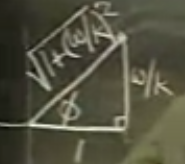
\includegraphics[height=3cm]{7_4.png}

Aradaki aci $\phi$, yani $arg(1+i(w/k)) = \phi$. 

Kompleks sayilarda bir kural soyledir, eger kompleks sayi 1'i boluyorsa,
aci degeri negatiflenir, ayrica mutlak (absolute), yani $r$ degeri, $1/r$
haline gelir, o zaman

\[ \frac{1}{1+i(w/k)} = A e^{-i\phi} \]

Peki A nedir? A ustteki ucgenin hipotenusu boleninde yer alan $1 /
\sqrt{1+(w/k)^2}$. 

\[ A e^{-i\phi} = \frac{1}{\sqrt{1+(w/k)^2}} e^{-i\phi}\]

Artik $\tilde{y}$'yi yazabiliriz. $Ae^{-i\theta}$ ve $e^{i\omega t}$'yi biraraya koyarsak

\[ \tilde{y} = A e^{i\omega t - i\phi} \]

\[ = \frac{1}{\sqrt{1+(w/k)^2}} e^{i(\omega t - \phi)} \]

Reel sonuc icin kompleks sistemden reel'e donuyoruz. Reel kisim kartezyen
formda $cos$ altinda olan terimdir, $sin$ kismini atariz, o zaman

\[ y_1 = \frac{1}{\sqrt{1+(w/k)^2}} cos(\omega t - \phi) \]

$\phi$'nin formulu nedir? Ustteki resme gore $\phi = tan^{-1}(w/k)$.

$cos(\omega t - \phi)$ baglaminda bakarsak $\phi$'ye faz gecikmesi de
denebilir, cunku $\phi$ olmadan $cos$ egrisinin nasil olacagini biliyoruz,
$\phi$ eklenince bu $cos$ egrisine bir gecikme etkisi yapacaktir.

Ekler

Teori: Alttaki denklem

$y' + ky = kq_e(t)$

icin girdi $q_e(t)$, $\cos \omega t$ olarak veriliyor. Biz problemi
komplekslestiriyoruz, ve $e^{i\omega t}$ ibaresinin reel tarafinin
kullaniyoruz cunku bu ibare Euler formulunun bir parcasi. O zaman elimizde
su var

$y' + ky = k e^{i \omega t}$

Fakat sonuc ta komplekslesecegi icin notasyonu $y$'den $\tilde{y}$'ye  degistiriyoruz,

$\tilde{y}' + k\tilde{y} = k e^{i \omega t}$

kompleks cozum $\tilde{y} = y_1 + iy_2$. Iddiamiz $\tilde{y}$'yi bulursak,
o zaman $y_1$ ilk, orijinal ODE'yi de cozer.

Ispat

$\tilde{y} = y_1 + iy_2$ ifadesini komplekslesmis ODE icine koyuyoruz.

$(y_1 + iy_2)' + k(y_1 + iy_2) = k e^{i\omega t}$

$y_1' + iy_2' + ky_1 + kiy_2 = ke^{i\omega t}$

Reel ve kompleks sayilari yanyana olacak sekilde grupluyoruz

$(y_1+ky_1) + i(y_2' + ky_2) = ke^{i\omega t}$

Ve goruyoruz ki ustteki denklemin sol tarafi icindeki reel kisim
$(y_1+ky_1)$, orijinal ODE'nin ($y$ icin $y_1$ kullanilirsa olacagi) sol
tarafi ile tipatip ayni, ayrica ustteki denklemin sag tarafinin reel kismi
$k \cos \omega t$, orijinal ODE'nin sag tarafina esit. Yani bekledigimiz
cozum sol tarafta ortaya cikinca, sag tarafta girdi olarak verdigimiz seyi
aynen goruyoruz. 


\end{document}


